\newpage
\chapter{Marco teórico}
La espectroscopia estudia la interacción entre la radiación electromagnética y la materia,en astronomía esta radiación es emitida por estrellas y otros objetos celestes y al ser dispersada brinda mucha información de la fuente que la genero.\\
Para el caso del espectro visible esta Luz puede ser dispersada usando un prisma mediante el fenómeno de refracción o usando una rejilla de difracción, estos espectros dan información importante de las características físicas del objeto que las emite,están directamente relacionadas con la temperatura superficial del objeto así como con su composición química. Usando Efecto Doppler se puede tener información de la velocidad de rotación y traslación además de densidad y presión. \cite{utilidad}\\

\section {Principios de la espectroscopia.}
Todo elemento que  irradie luz presenta en esta luz información detallada de las propiedades constituyentes de dicho elemento así como su temperatura, esta luz esta compuesta de múltiples longitudes de onda que son separadas y se pueden observar en un sensor ccd en forma de linea espectral, que es la distribución de  la intensidad en función de la longitud de onda o la frecuencia  de luz dispersada.

\subsection {Espectros y lineas espectrales.}

Históricamente las lineas espectrales fueron llamadas así ya que se  presenta como lineas de obscuridad o luminosidad en la salida de un espectroscopio luego de la dispersión, por esto la forma de las lineas dependen del instrumento que se este utilizando.\\
Estas lineas son de origen cuántico y se generan por la transición de 2 niveles de energía, estos puede dividirse en 3 tipos,las lineas espectrales continuas ,de emisión y las de absorción.\cite{troccoli}


\textbf{Espectro Continuo:}
Se define un espectro continuo cuando la franja de colores  pasa de un color a otro sin ninguna interrupción de franjas negras entra color y color como se presente en la figura 1, se puede observar esto con la luz blanca y en general cualquier solido o gas sometido a altas presiones o temperaturas presente un espectro continuo.


\begin{figure}[htb!]
\centering

\includegraphics[width=0.7\textwidth]{images/1.png}
\caption[Espectro continuo.]{Espectro continuo.\cite{libro}}
 \label{fig2}
\end{figure}

\textbf{Espectro de emisión :} Un gas a baja presión y excitado a altas temperaturas produce un espectro de emisión,estos espectros constan de rayas de diversos colores separadas por amplias zonas  negras en las que no se observa luz ver figura 2. Este tipo de espectro se da cuando los electrones en los átomos de estos gases excitados absorben energía de la fuente que los esta excitando  y saltan a orbitas superiores , la emisión tiene lugar cuando los electrones caen a niveles mas bajos emitiendo este exceso de energía en forma de fotones con una frecuencia característica propia de cada elemento.


 \begin{figure}[htb!]
\centering
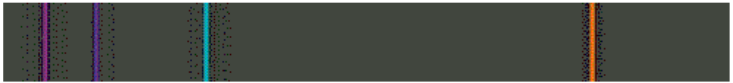
\includegraphics[width=0.7\textwidth]{images/2.png}
\caption[Descripción versión comprimida]{El espectro de emisión del hidrógeno \cite{articulo1}}
 \label{fig3}
\end{figure}


\textbf{Espectro de absorción :} Este tipo de espectro se da cuando se hace pasar luz blanca a través de un gas frío a baja presión, el espectro que se observa presenta un fondo de color con franjas negras, con la característica principal de que las lineas de absorción aparecen en el mismo lugar que las lineas de emisión.\\
En astronomía las fuente luminosa generalmente es una estrella, la luz proveniente de la estrella atraviesa capas de gas propia de la atmósfera, las lineas de absorción dependerán estrictamente de la composición química del gas, esta absolverá fotones de una u otra longitud de onda dejando las franjas obscuras características de espectro de absorción.


\begin{figure}[htb!]
\centering
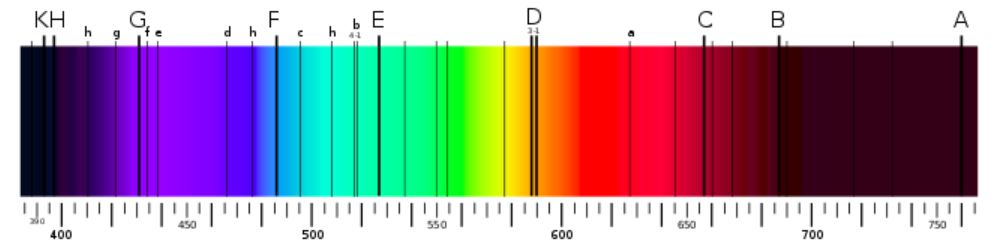
\includegraphics[width=0.7\textwidth]{images/3.png}
\caption[Descripción versión comprimida]{Espectro solar en el que se aprecian las líneas principales de von Fraunhofer. \cite{articulo1}}
 \label{fig4}
\end{figure}

%falta citar de https://culturacientifica.com/2019/08/13/los-espectros-de-absorcion-de-los-gases/

Los anteriores espectros tienen su explicación en las leyes de kirchof  que se presentan a continuación.

-Un espectro continuo se produce por un un solido incandescente o un gas a alta presión.

-Un espectro de emisión se produce por un gas incandescente a baja presión.

- Cuando se hace pasar luz blanca a través de un gas a baja presión y baja temperatura se produce un espectro de emisión.

\subsection {Radiación de cuerpo negro}
Es bien conocido el fenómeno por el cual todos los cuerpos que se encuentran por encima del cero absoluto presentan radiación electromagnética, a altas temperaturas se habla de incandescencia pues las longitudes de onda de emisión se encuentran en el espectro visible (entre 400 y 700 nm) aun a bajas temperaturas  el objeto seguirá irradiando pero ahora en el infrarroja (longitudes de onda superiores a 700 nm).\cite{libro2} \\
Kirchoff propuso en 1860   una hipótesis  de radiación para los cuerpo en equilibrio , la denomino radiación de cuerpo negro, esta muestra como la radiación tiene un patrón regular que depende de la temperatura.Mas tarde  Wein y Plank  hicieron el desarrollo matemático e este fenómeno, que se puede modelar como:


\begin{equation}
    \lambda_{max}=\frac{0.002898}{T}
\end{equation}


Donde $ \lambda$ es la longitud de onda máxima emitida por el cuerpo y T es la temperatura en grados Kelvin.\\

\textbf{Ley de desplazamiento de Wien:}Durante el año 1893 Wien basándose en argumentos estadístico dedujo que la distribución normal de radiación, como era conocida hasta la fecha se modelaba  con la expresión:  


\begin{equation}
    I(\nu,T)=\nu^3 f \left(\frac{\nu}{T}\right)
\end{equation}


Donde $f\left(\frac{\nu}{T}\right)$ es desconocida pero solo puede depender de $\nu$ y de T.\\
Sin embargo Wien usando los datos de los experimentos realizados en la época pudo llegar a una expresión mas detallada para la ecuación  (2).  


\begin{equation}
    I(\nu,T)= a \nu^{3} e^{-b(\frac{\nu}{T})}
\end{equation}{}


Donde a y b son constantes que se determinan durante el experimento.\\
Esta expresión modelaba muy bien los experimentos  reproducidos en la época y daba una explicación satisfactoria a los resultados empíricos que demostraban que la frecuencia de radiación mas intensa emitida por un cuerpo negro $\nu_{max}$ aumenta linealmente con la temperatura.

\begin{figure}[htb!]
\centering
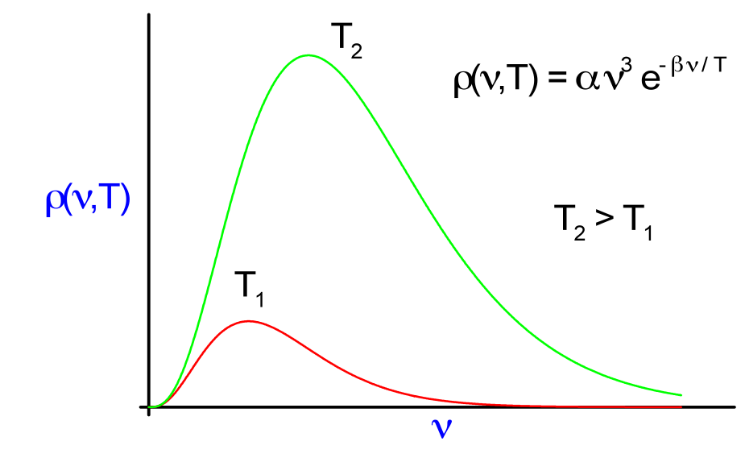
\includegraphics[width=0.6\textwidth]{images/5.png}
\caption[Descripción versión comprimida]{Wien propuso la expresión para la distribución normal de radiación que predice el pico de la distribución de corriente lineal con la la temperatura T.\cite{plank}}
 \label{fig1}
\end{figure}

\textbf{La deducción de Planck:}Para el año 1900 Otto Lummer y Ernst Pringsheim junto con otros 2 investigadores Heinrich Rubens y Ferdinand Kurlbarm realizaron múltiples experimentos y notaron que la ecuación de Wien (1.3) no concordaba con los experimentos a frecuencias bajas, a estas frecuencias la distribución normal de radiación notaron que eran directamente proporcional al cuadrado de la frecuencia por la temperatura.

\begin{equation}
    I(\nu,T) \sim \nu^{2} T
\end{equation}{}






%http://www.quimicafisica.com/radiacion-cuerpo-negro-hipotesis-planck.html





\subsection {Diagramas de Hertzsprung-Russell}


La espectroscopia permitió la construcción del diagrama Hertzsprung-Russell, el cual se desarrollo inicialmente en la Universidad de Harvard.
Este diagrama muestra la etapa de evolución de las estrellas con las líneas espectrales que señala el estado de los elementos químicos presentes en ellas. La figura 2.3 muestra como se relacionan las estrellas en tamaño, color, luminosidad, clase espectral y la magnitud absoluta. Cada punto en este diagrama representa una estrella en el firmamento, cuya magnitud y clase espectral absoluta han sido determinadas. Los datos se agrupan en: estrellas de secuencia principal, supergigantes, gigantes y enanas
blancas.


%\subsection {Lineas de franhofer}


